\subsubsection{Kiến trúc vi dịch vụ (Microservice Architecture)}

Kiến trúc vi dịch vụ chia bài toán thành các thành phần nhỏ hơn được gọi là các dịch vụ.
\begin{itemize}

\item Mỗi dịch vụ tập trung vào một khả năng kinh doanh cụ thể.

\item Các dịch vụ độc lập và giao tiếp với nhau thông qua hạ tầng mạng.
\end{itemize}

Một số lợi ích của Microservice:

\begin{itemize}
\item Mỗi dịch vụ có các biến bí mật (secret) riêng.
\item Không cần cài các thư viện, các phụ thuộc với dịch vụ không dùng
\item Đa dạng ngôn ngữ lập trình khác nhau theo từng logic của từng dịch vụ
\item Phân chia tài nguyên cho từng dịch vụ (ví dụ Heroku giới hạn RAM, AI cần GPU)
\item Giảm thời gian quá trình kiểm thử vì mỗi dịch vụ có nghiệp vụ khác nhau

\item Vì các dịch vụ độc lập, dễ dàng triển khai
\item Tăng khả năng mở rộng hệ thống

\end{itemize}

% Nhược điểm Microservice ???
% Nhược điểm Microservice ???
% Nhược điểm Microservice ???
% Nhược điểm Microservice ???
% Nhược điểm Microservice ???
% Nhược điểm Microservice ???
% Nhược điểm Microservice ???
% Nhược điểm Microservice ???
% Nhược điểm Microservice ???
% Nhược điểm Microservice ???
% Nhược điểm Microservice ???

\begin{figure}[H]
\centering
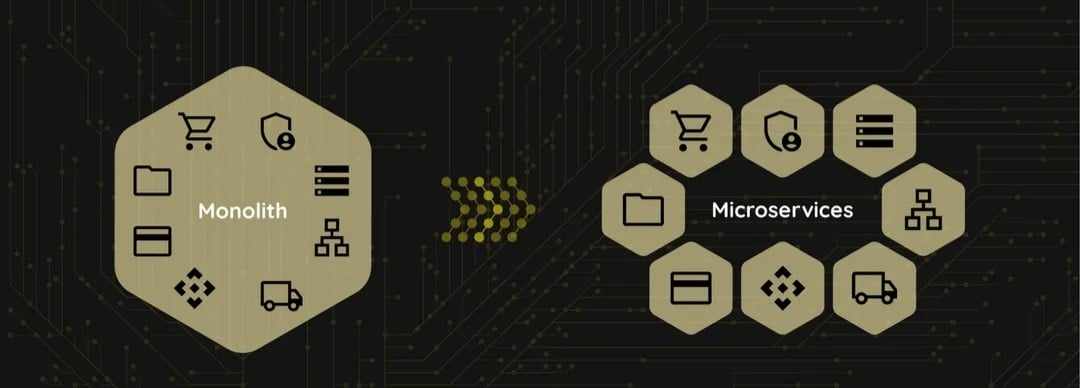
\includegraphics[scale = 0.3]{pictures/mono.png}
\caption{Giới thiệu Microservice}
\end{figure}

Tổng quan các dịch vụ của dự án:

\begin{figure}[H]
\centering
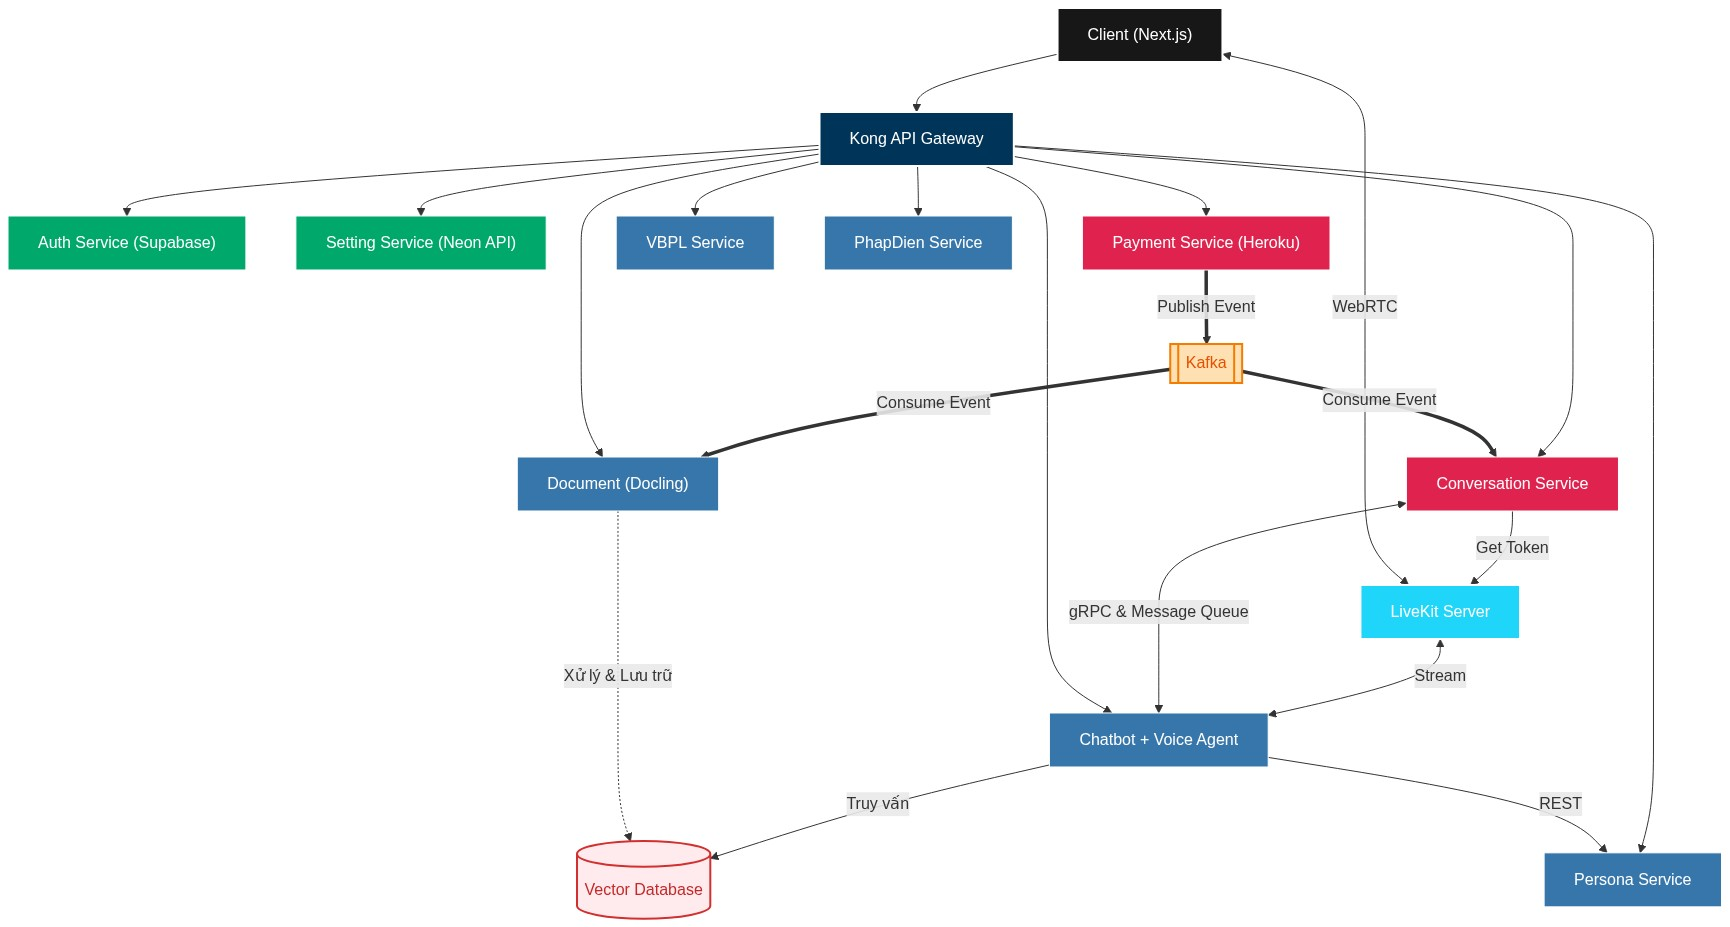
\includegraphics[scale = 0.24]{pictures/MSA.png}
\caption{Tổng quan các dịch vụ của dự án}
\end{figure}
